\section{Delivery-time minimization}
\label{sec:method}

\subsection{Running example and enforcement boundary}
The user asks for one refund, preferring the wallet and authorizing the bank as fallback if the wallet is unavailable. A trusted status response initially marks the wallet unavailable and the bank available. The agent proposes the bank route. Its pending account verification step needs an account reference and an owner reference. Before those references enter model context, the wallet recovers. Both backends deny the old request and give the agent the same safe recovery options. The agent then proposes the wallet route, reads its wallet reference and obtains the required confirmation before executing the refund (Figure~\ref{fig:refund-sequence}).

The agent controls which actions and fields it requests. The connector controls which raw values cross into model context. Above that boundary, both backends expose the same user authorization, route preferences, status queries, approval policy and recovery interface. Below it, the \emph{refreshed route table} composes reusable route recipes and evaluates route, prerequisite and field rules from the current snapshot. The \emph{contract verifier} derives step requirements from tool contracts, binds a read grant to its supporting evidence and revalidates it at delivery. The stores and trusted state interface are shared. Figure~\ref{fig:mechanism} locates each decision and the common release point.

\begin{figure*}[t]
\centering
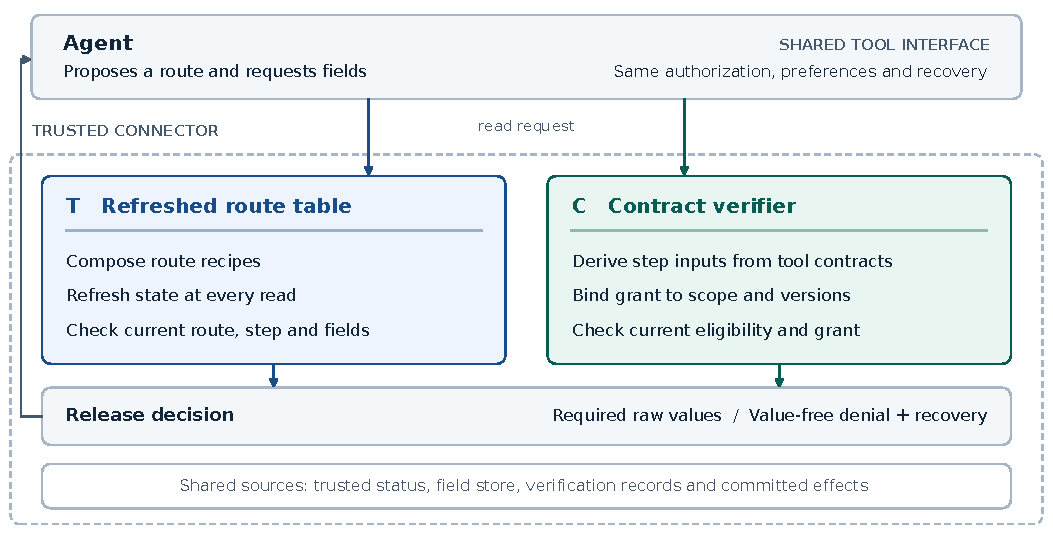
\includegraphics[width=\textwidth]{figures/backend-comparison.pdf}
\caption{Both backends enforce the same delivery boundary. The route table derives permission anew from the current snapshot at every read. The contract verifier additionally checks that the evidence and values bound to an earlier grant still match. Each backend returns permitted values or a value-free denial through the same tool interface.}
\label{fig:mechanism}
\end{figure*}

\subsection{Selecting a plan with incomplete evidence}
A tool step $a$ declares required and produced artifacts, required raw fields $R_a$ and business predicates. A plan joins steps that can achieve the remaining goals from the available artifacts. $\mathcal P_U$ contains only plans whose tools and fields fall within the user's authorization $U$. The route table obtains candidates from configured recipes. The contract backend derives them from artifact production and consumption.

Let $B(p)$ be the required literals for plan $p$. The evidence view $E_t$ contains current known true literals. If neither a literal nor its negation appears, its truth is unknown. Let $\overline{B(p)}$ be the pointwise negation of $B(p)$. The possible and proven sets are
\begin{align}
P_t &= \{p\in\mathcal P_U : E_t\cap\overline{B(p)}=\emptyset\},\label{eq:possible}\\
K_t &= \{p\in P_t : B(p)\subseteq E_t\}.\label{eq:proven}
\end{align}
Let $\rho(p)$ order plans by user preference and, if configured, by disclosure cost as a tie-breaker. Lower is better. With $r_t=\min_{p\in K_t}\rho(p)$ and $\min\emptyset=+\infty$, the unresolved higher-priority set and the admissible plans are
\begin{align}
Q_t &= \{p\in P_t\setminus K_t : \rho(p)<r_t\},\label{eq:unresolved}\\
A_t &=
\begin{cases}
\{p\in K_t:\rho(p)=r_t\}, & Q_t=\emptyset,\\
\emptyset, & Q_t\ne\emptyset .
\end{cases}\label{eq:admissible}
\end{align}
The agent proposes a plan. The backend checks whether it is in $A_t$. If $Q_t$ is nonempty, status evidence for those unresolved plans must be obtained first. For example, confirmed bank availability alone does not establish fallback while wallet availability is unknown. Evidence of wallet unavailability excludes the wallet plan and can make the bank plan admissible.

\subsection{Deciding what to release}
Write $X_t=(E_t,\eta_t,\nu_t,H_t,M_t,L_t)$ for a trusted snapshot. Here $\eta_t$ and $\nu_t$ map predicates and values to versions with fresh identifiers on update, $H_t$ holds verification records, $M_t$ holds fields already delivered at their current version, and $L_t$ is the ledger of committed effects. Let $s$ denote a plan session on resource $r$, with plan $p_s$. For an enabled step $a$ in that session, the missing raw fields are
\begin{equation}
D_t(a)=R_a\setminus M_t.\label{eq:missing}
\end{equation}
An enabled step is pending, has its prerequisites satisfied and respects confirmation requirements applicable at that step. For the two backends we use the following common release predicate. $S$ is the set of fields in the request, after rejecting duplicate field identifiers. Scope checks the resource, session and step.
\begin{align}
\mathrm{Allow}_t(r,s,a,S)={}&
\mathrm{Scope}(r,s,a) \land p_s\in A_t \notag\\
 &{}\land\mathrm{Enabled}_t(s,a)
 \land S=D_t(a).\label{eq:common-guard}
\end{align}
The route table refreshes $X_t$ for each read, resolves the matching route recipe and applies Eq.~\eqref{eq:common-guard} using its field and prerequisite rules. A contract read first obtains a single-use grant
\begin{equation}
g=(r,s,a,D_i(a),\sigma_s,\nu_i|_{D_i(a)}),\label{eq:grant}
\end{equation}
where $i$ is the issue time and $\sigma_s$ holds the predicate versions captured for the accepted session. This includes relevant evidence excluding a preferred alternative. The reference implementation conservatively tracks known predicates across permitted plans. For redemption, in addition to Eq.~\eqref{eq:common-guard}, the request must satisfy
\begin{align}
 &\mathrm{Unused}(g)\land\mathrm{Match}(g,r,s,a,S)\notag\\
 &{}\land\eta_t|_{\mathrm{dom}(\sigma_s)}=\sigma_s
 \land\nu_t|_S=\nu_i|_S .\label{eq:grant-valid}
\end{align}
$\mathrm{Match}$ binds the request to the grant's scope and field set. The current plan check remains necessary because resolving a previously unknown predicate can change $A_t$ without changing an entry recorded in $\sigma_s$. A tracked change can also invalidate the grant while the same plan remains admissible. The refreshed table can allow such a read when the current step and requested fields still satisfy its rules.

\begin{figure*}[t]
\centering
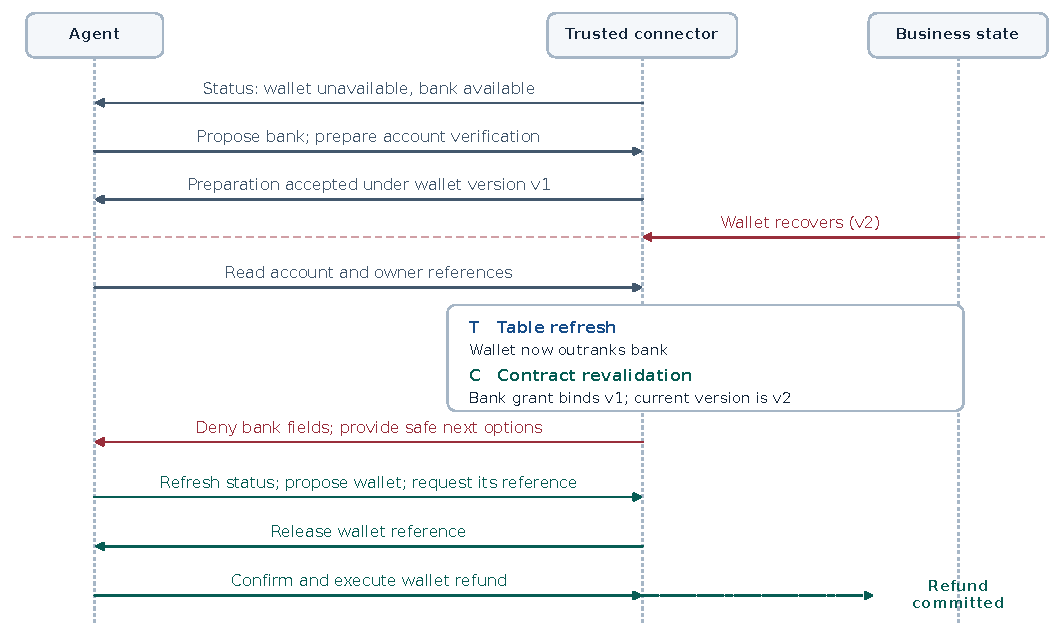
\includegraphics[width=\textwidth]{figures/refund-sequence.pdf}
\caption{Worked refund trace, with the two backend outcomes shown as alternatives for the same request. Wallet availability changes from false to true before delivery. The table excludes the now lower-priority bank route. The contract verifier also sees that its grant binds the previous wallet version. Both return a denial without bank data. The agent proposes and completes the wallet route. Versions are illustrative.}
\label{fig:refund-sequence}
\end{figure*}

\subsection{Safety property}
\textbf{Proposition 1 (necessity at delivery).}
Assume (i) all raw reads in scope pass through the trusted connector, (ii) authorized routes and step-field rules faithfully specify business prerequisites and required fields, and (iii) the authorization check and value release are evaluated against the same current snapshot. If either backend releases any raw fields for a step, the step is enabled on a currently admissible plan and the released fields are exactly its missing required set $D_t(a)$. In contract mode, changing a tracked predicate or bound field version invalidates the old grant.

\emph{Proof.} For every release, Eq.~\eqref{eq:common-guard} requires membership in $A_t$, scope, step eligibility and equality to $D_t(a)$. By (iii), the released values correspond to that same snapshot. A failed conjunct yields a denial with no raw values. The contract verifier also requires both version equalities in Eq.~\eqref{eq:grant-valid}. A changed bound version makes its equality false. In the refund trace, the wallet recovery removes the bank plan from $A_t$ and changes the wallet predicate version in the bank grant. Thus either backend denies the old read.\hfill\rule{.6ex}{.6ex}

The evaluated simulator processes validation and delivery sequentially. A concurrent connector needs an atomic conditional read or an equivalent version-checked transaction before this property applies. The result concerns release of raw values via the connector. It leaves inference from status signals, reuse of already delivered values and disclosure in model output outside the guarantee.

\subsection{Recovery after rejection}
A denial supplies a reason, valid artifacts already available and safe next options within $U$. It carries no newly read raw values. Let $X'$ be the refreshed state and $G$ the original goals. The shared recovery rule filters reusable records and current-value markers and replans against the ledger:
\begin{align}
H' &= \{h\in H : \mathrm{Valid}(h,X',r,U)\},\label{eq:reuse}\\
M' &= \{f\in M : \nu'(f)=\mathrm{SeenVersion}(f)\},\label{eq:seen}\\
G_{\mathrm{left}} &= G\setminus\mathrm{Done}(L).\label{eq:remaining}
\end{align}
Verification reuse requires the same resource and an allowed purpose, plus current relevant versions. Here $M'$ changes what may be treated as current by the connector. It does not erase earlier model context. The ledger stays fixed during replanning. Subsequent successful business operations can extend it. If no authorized continuation exists, the agent stops, or asks for new consent only when the shared approval policy permits it.

In the worked refund trace, the ledger has no committed refund when the bank read fails. The agent selects the wallet and issues new calls, and only the wallet reference is delivered. In a separate reuse case, an earlier identity verification can carry across the route change if Eq.~\eqref{eq:reuse} holds. The scripted adapters implement reuse for supported verification records and business effects.

\begin{table}[t]
\small
\centering
\begin{minipage}{.98\columnwidth}
\hrule\vspace{4pt}
\textbf{Algorithm 1. Select and read}\\[2pt]
\textbf{Select:} derive candidates for remaining goals\\
\quad compute $Q_t$ and $A_t$ (Eqs.~\ref{eq:unresolved}--\ref{eq:admissible})\\
\quad \textbf{if} $Q_t\ne\emptyset$: request status evidence\\
\quad \textbf{if} $A_t=\emptyset$ and $Q_t=\emptyset$: report no route\\
\quad validate the agent's proposed plan against $A_t$\\
\textbf{Prepare (contract):} issue the grant (Eq.~\ref{eq:grant})\\
\textbf{Read:} obtain the delivery snapshot\\
\quad table: resolve the current recipe and check Eq.~\eqref{eq:common-guard}\\
\quad contract: check Eqs.~\eqref{eq:common-guard} and \eqref{eq:grant-valid}\\
\quad \textbf{if} a check fails: deny with safe feedback\\
\quad release permitted values and consume any grant
\vspace{4pt}\hrule
\end{minipage}
\end{table}

\begin{table}[t]
\small
\centering
\begin{minipage}{.98\columnwidth}
\hrule\vspace{4pt}
\textbf{Algorithm 2. Continue after a denied read}\\[2pt]
\textbf{Agent:} refresh status using a permitted tool\\
\quad use the backend's valid records and remaining goals\\
\quad query unresolved evidence if needed\\
\quad \textbf{if} no authorized continuation: stop or seek consent\\
\quad propose a plan and issue fresh calls for its missing inputs\\
\quad confirm as required, then call the business action\\
\textbf{Backend:} check prerequisites and record committed effects
\vspace{4pt}\hrule
\end{minipage}
\end{table}
